\documentclass{whutmod}
\usepackage[linesnumbered,ruled,lined]{algorithm2e}
\bibliographystyle{unsrt}
\team{10}
\membera{刘子川}
\joba{编程}
\memberb{程宇}
\jobb{建模}
\memberc{祁成}
\jobc{写作}
\hypersetup{
	colorlinks=true,
	linkcolor=black,citecolor=black
}


\newcommand{\upcite}[1]{\textsuperscript{\cite{#1}}}
%%%%%%%%%%%%%%%%%%%%%%%%%%%%%%%%%题目%%%%%%%%%%%%%%%%%%%%%%%%%%%%%%%%%%%%
\title{基于xxxxxxxx模型}
\tihao{1} 

\begin{document}

%	\maketitle
%	\thispagestyle{empty}

\begin{center}
	\vspace{4pt}
	{\normalfont \LARGE \textbf{基于灰色马尔可夫与Leslie模型的中国人口预测} }\par
	\vspace{4pt}
	\noindent
\end{center}

%%%%%%%%%%%%%%%%%%%%%%%%%%%%%%%%%摘要%%%%%%%%%%%%%%%%%%%%%%%%%%%%%%%%%%%%
	\begin{abstract}
		本文建立了我国人口增长的预测模型,对各年份全国人口总量增长的中短期和长期趋势作出了预测,并对人口老龄化、人口抚养比等一系列评价指标进行了预测。最后提出了有关人口控制与管理的措施。
		\vspace{7pt}	%空格
		
		针对问题一,在传统\textbf{灰色预测模型}的基础上,利用\textbf{马尔科夫链}校正预测结果误差, 得到\textbf{灰色马尔科夫模型}并进行预测。本组首先建立传统 GM(1,1) 模型,预测分析 2001-2020 年全国人口总数。再通过马尔科夫模型,计算预测残差的期望 值。最后利用残差期望校正传统灰色预测的固有偏差。预测得到2021-2030年全国人口总数并分析其人口结构变化。该模型预测\textbf{误差低于7\%},\textbf{NSE值趋近于1},说明模型可信度很高。
	
		\vspace{7pt}	%空格
	
		针对问题二,建立基于动力系统城乡迁移人口流动规律的\textbf{带有迁移项的$Leslie$人口发展模型},考察离散化的时间节点和人群年龄分布。在经典$Leslie$矩阵法的基础上,\textbf{引入城乡迁徙率},考虑城市化进程对人口发展规律的影响。单独分析死亡率、出生率、迁移率对人口结构与人口总量发展的影响,综合三者影响得到含未知参数的人口更新方程。之后设计并使用\textbf{免疫差分进化算法},求解人口更新方程中人口迁移率等未知参数。结果表明预测出将来我国育龄妇女人数与生育旺盛期育龄妇女人数,得到育龄妇女人数在短期内将达到高峰,随后又下降的趋势。对求解结果进行误差分析与灵敏度分析,考察死亡项、生育项、迁移项六个参数对总人口发展的影响。
		\vspace{7pt}	%空格
	
		针对问题三,结合问题 1 和问题 2 的分析,为相关部门提供一份在人口结构政策调控等方面的可行性报告。
		\vspace{7pt}	%空格
	
		本文的优点为:一、利用马尔可夫模型改进后的灰度预测值 与实际值拟合度更高,波动性保持一致;二、 结合了人口迁移的实际特点改进了 Leslie人口模型,且使用免疫差分进化算法估计参数, 使得预测模型更贴近于我国的实际情况。
		
		\keywords{
			灰色预测\quad
			马尔可夫链\quad	
			Leslie人口增长模型\quad
			免疫差分进化\quad
		}
	\end{abstract}


%%%%%%%%%%%%%%%%%%%%%%%%%%%%%%%%%目录%%%%%%%%%%%%%%%%%%%%%%%%%%%%%%%%%%%%
%	\thispagestyle{empty}
%	\tableofcontents
%	\setcounter{page}{0}                                               
%	\newpage	%换页符
	

	
	\section{问题重述}	
		\subsection{问题背景}
		人口的数量和结构是影响经济和社会、发展关系到人口延续和社会进步的重要因素。计划生育国策的制定对人口总量、生育质量控制有积极且深刻的影响,但带来人口老龄化、养老、劳动力供需等一系列问题。但是随着人口结构的快 速转变,计划生育带来的负面效应也逐渐显现,面对生育水平持续降低、劳动力短缺、老龄化程度不断加剧等问题,为此国家于2013年11月放开单独家庭二孩生育政策,两年后于2015年12月27日实施全面二孩政策。逐步调整完善生育政策,并完善相关生育政策保障体系,进一步调整社会结构,促进社会经济的发展。生育政策调整以来,学术界通过“预期”与生育数据统计结果对比认为“二孩”政策的效应不够理想。因此,需要建立依赖生育模式、生育率、死亡率和性别比等多个基本因素的人口问题理论和模型,综合考虑新时代中国社会经济水平发展,政策改变及人的观念、社会文化习俗。

	
		\subsection{问题概述}
		    围绕相关附件和条件要求,研究人口结构变化分析及预测,依次提出以下问题:
				 
			
			\textbf{问题一:}搜集“二孩”政策开放以来某地区或区域人口数据,分析“二孩”政策对人口结构变化的影响。
			
			\textbf{问题二:}建立适当的人口数学模型,对某地区或区域人口结构及变化进行预测分析。
			
			\textbf{问题三:}结合问题 1 和问题 2 的分析,为相关部门提供一份在人口结构政策调控等方面的可行性报告。

	
	\section{模型假设}
		\begin{itemize}                                             
		\item [(1)]考虑出生率时,忽略女性妊娠期与一年离散化时间节点步长的差值带来的时滞效应。
		\item [(2)]假设全国人口分布是封闭动力系统,只考虑境内城乡迁徙率,忽略海外留学、移民对人口分布的影响。
		\item [(3)]假设出生率、死亡率、迁徙率对人口分布的影响独立,且具有可加性。
		\item [(4)]假设人口与经济发展无关,其它影响因素可以忽略不计。 
		\end{itemize}

		
	\section{符号说明}
		\begin{table}[H]
		\centering
		\setlength{\tabcolsep}{5mm}
		\begin{tabular}{cc}
			\toprule[1.5pt]
			\multicolumn{1}{m{1cm}}{\centering 符号} & \multicolumn{1}{m{13cm}}{\centering 说明} \\
			\midrule[1pt]		
			$p_i(t)$  & 研究时间阶段的第$t$年满$i$周岁,但不满$i+1$周岁的人口数 \\ 
			$b_r$  & 满$r$周岁,但不满$r+1$周岁的人口出生率  \\ 
		   	$v_i$  & 第$i$年净迁徙人数  \\ 
		   	$\beta(t)$  & 女性平均生育率函数  \\ 
		   	$k_i(t)$  & 满$i$周岁,但不满$i+1$周岁女性占总人口比率 \\ 
		   	$d_i(t)$  & 第$t$年年龄为$i$岁的人群死亡率 \\ 
			\bottomrule[1.5pt]
		\end{tabular}
		\begin{tablenotes}
		\item 注:表中未说明的符号以首次出现处为准
		\end{tablenotes}
		\end{table}

		
			\section{问题一模型的建立与求解}
		\subsection{问题描述与分析}
		
		问题一要求根据中国数据统计局中2001年至2020年的全国人口相关数据,运用数学模型对2020年至2030年我国每年人口总数预测。本组首先选择合适的指标后建立\textbf{灰色预测}模型,预测分析2001-2030年我国每年人口总数。再通过\textbf{马尔科夫模型},由2001-2020年的数据模拟残差在各个区间的分布,计算2021-2030年预测残差的期望值。最后将预测结果与残差期望做差,\textbf{校正}传统灰色预测的固有偏差,经过两种模型的结合达到科学预测人口总数的未来发展趋势的目的,并通过人口总数的变化分析“二胎政策”对人口结构的改变。其思维流程图如图~\ref{lcdadat}~所示:
		
		\begin{figure}[H]
			\centering
			
\includegraphics[width=\textwidth]{figures/lctc.png}
			\caption{问题一思维流程图}\label{lcdadat}
		\end{figure}
%		
		
		\subsection{模型的建立}
		\subsubsection{灰度预测GM(1,1)}
		设2001-2020年总发病人数为时间序列:
		\begin{gather*}
		X^{(0)}=[x^{(0)}(1),x^{(0)}(2),\cdots,x^{(0)}(20)],
		\end{gather*}
		通过一次累加生成1-AGO序列:
		\begin{gather*}
		X^{(1)}=[x^{(1)}(1),x^{(1)}(2),\cdots,x^{(1)}(20)],
		\end{gather*}
		式中:$x^{(1)}(k)=\sum_{i=1}^{k}x^{(1)}(i),k=1,2,\cdots,20$。
		
		根据1-AGO序列建立微分方程为:
		\begin{gather}\label{333}
		\frac{d X^{(1)}}{dt}+a X^{(1)} = u,
		\end{gather}
		式中:$a$称为发展灰度,$u$称为内生控制灰度。设$\widehat{\alpha}$为待估参数向量,且$\widehat{\alpha }=[a,u]^T$,利用最小二乘法求出:
		\begin{gather*}
		\widehat{\alpha }=(B^TB)^{-1}B^{T}Y_{n}.
		\end{gather*}
		
		
		求解方程(~\ref{333}~),可得第$k+1$年中国人口总数的\textbf{人口预测模型}为:
		
		\begin{gather}
		\widehat{X}(k+1)=[X^{(0)}(1)-\frac{u}{a}]e^{-ak}+\frac{u}{a},k=1,2,\cdots,30,
		\end{gather}
	
		\subsubsection{马尔科夫模型校正}
		利用马尔科夫模型对GM(1,1)预测误差项的状态及状态概率进行预估,并利用预测状态的期望值对GM(1,1)预测值进行修正。用2001-2020年预测数据与真实数据残差进行状态划分,设残差序列为:
		\begin{gather*}
		\varepsilon =[\varepsilon(1) ,\varepsilon(2), \cdots,\varepsilon(20)].
		\end{gather*}
		
		最大残差绝对值为$\delta _{max}=\underset{1\leqslant i\leqslant20 }{max}\left | \varepsilon(i) \right |$,将预测误差化均分为三个状态。令$\lambda =\frac{\delta _{max}}{6}$。状态分别为$E_{1}:(-3\lambda,-\lambda)$、$E_{2}:(-\lambda,\lambda)$和$E_{1}:(\lambda,3\lambda)$。其中初始状态概率向量计算公式为:
		
		\begin{gather}
		\left\{\begin{matrix}
		p_{Ek}=\frac{n_{Ek}}{20},\\
		t_{0}=[p_{E1},p_{E2},p_{E3}],
		\end{matrix}\right.
		\end{gather}
		式中:$n_{Ek}$是状态$E_{k}$在2001-2020年内出现的次数,以状态$E_{k}$出现的频率代替其出现的概率$p_{Ek}$。且构建状态转移矩阵为:
		\begin{gather*}
		P=\left(\begin{array}{lll}{P_{11}} & {P_{12}} & {P_{13}} \\ {P_{21}} & {P_{22}} & {P_{23}} \\ {P_{31}} & {P_{32}} & {P_{33}}\end{array}\right),
		\end{gather*}
		式中:$P_{ij}$是由状态$E_{i}$经过一个时期转移到$E_{j}$的转移概率。
		
		即马尔科夫模型可表示为:	  
		\begin{gather}
		t_{k+1}=t_{k} \cdot p.
		\end{gather}
		
		设状态区间的中间值分别为$\overline{E}_{1}$、$\overline{E}_{2}$和$\overline{E}_{3}$,即第k年GM(1,1)的误差期望为:
		\begin{gather}
		\eta =\begin{bmatrix}
		p_{E1} & p_{E2} & p_{E3}
		\end{bmatrix} \cdot\begin{bmatrix}
		\overline{E}_{1}\\ 
		\overline{E}_{2}\\ 
		\overline{E}_{3}
		\end{bmatrix}.
		\end{gather}
		
		当第$k$年的人口总数的GM(1,1)预测值为$\widehat{x}(k)$时,\textbf{修正后的灰色马尔可夫组合预测}模型$\overline{x}(k)$可以记作:
		\begin{gather}
		\overline{x}(k) =\widehat{x}(k)-\eta.
		\end{gather}
		\subsubsection{预测结果评价指标}
		均方根误差(RMSE)、平均相位误差绝对值(MAPE)和纳什效率系数(NSE)三者是常用来衡量预测结果的指标。RMSE能评价中国人口总数中高值的预测结果,其计算公式为:
		
		\begin{gather*}
		\operatorname{RMSE}=\sqrt{\frac{1}{n} \sum_{i=1}^{n}\left(y_{i}-y_{i}^{*}\right)^{2}},
		\end{gather*}
		均方根误差越小,表明模型可靠性越高,结果越准确。
		
		MAPE用来评价预测数据中平稳部分的预测结果,其计算公式为:
		\begin{gather*}
		\mathrm{MAPE}=\frac{1}{n} \sum_{i=1}^{n}\left|\frac{y_{i}-y_{i}^{*}}{y_{i}}\right| \times 100 \% ,
		\end{gather*}
		MAPE所求值为绝对值,是一个相对指标,当两个MAPE值进行比较时,值越小的说明模型可靠性越高。
		
		NSE可以用来评价模型的预测能力,其计算公式如下:
		\begin{gather*}
		\mathrm{NSE}=1-\frac{\sum_{i=1}^{n}\left(y_{i}-y_{i}^{*}\right)^{2}}{\sum_{i=1}^{n}\left(y_{i}-\overline{y}\right)^{2}}       ,
		\end{gather*}
		求得NSE值越接近$1$,表示模型质量越好,模型可信度越高。接近$0$,表示模拟结果接近观测值的平均水平,即总体结果可信,但模拟误差较大。远远小于$0$,则模型是不可信的。

		
		\subsection{灰色马尔可夫模型的求解}
		通过在中国数据统计局的数据下得到以下2001-2019年的全国人口总数、城乡人口及男女人口数目统计表。
		\begin{table}[H]
			\setstretch{1.4}  %设置表的行间距
			\centering		
			\caption{2001-2020年人口数量统计表(单位:万人)}\label{biadao1}
			\begin{tabular}{cccc}
				\toprule[2pt]
				\multicolumn{1}{m{2cm}}{\centering 年份}
				& \multicolumn{1}{m{3cm}}{\centering 人口}
				&\multicolumn{1}{m{2cm}}{\centering 年份}
				& \multicolumn{1}{m{3cm}}{\centering 人口}
				\\
				\midrule[1pt]
				2001 & 	121121&2011 &130756 \\ 
			2002	& 122389 & 2012 &131448  \\
				2003&  123626&  2013& 132129 \\
				2004& 124761 & 2014 &132802  \\
			2005	&125786  & 2015 & 133450 \\
			2006&126743  & 2016 &134091  \\
			2007& 127627 & 2017 &135040  \\
			2008&128453  & 2018 & 136072 \\
			2009&  129227&  2019& 136782 \\
		2010 & 	129988&2020 &137462 \\ 
				\bottomrule[2pt]	
			\end{tabular}
		\end{table}
		
		通过 GM(1,1) 计算 2001-2020 年人口总数预测值得到灰度预测解如下:
				\begin{gather*}
		\widehat{w}^{(k+1)}  = 26851348.3155e^{0.0049807k}  -2671798.3155 ,k=1,2,\cdots,20,
		\end{gather*}
		其误差状态区间如表 1 所示:
			  	 \begin{table}[H]
			\centering\caption{人口总数状态区间划分}\label{ff}
			\begin{tabular}{cccc}
				\toprule[1.5pt]
				\multicolumn{1}{m{2cm}}{\centering 状态}
				& \multicolumn{1}{m{3cm}}{\centering $E_{1}$}
				& \multicolumn{1}{m{3cm}}{\centering $E_{2}$}
				& \multicolumn{1}{m{3cm}}{\centering $E_{3}$}
				\\
				\midrule[0.5pt]
				残差区间 &  $[-66389,-22130]$  &$(-22130,22130]$ & $(22130,66389]$   \\ 
				\bottomrule[1.5pt]	
			\end{tabular}
		\end{table}  
		根据误差区间范围,将 2001-2020 年人口总数预测值归类于误差区间如表 2 所示:
		 \begin{table}[H]
			\centering\caption{人口总数误差状态区间}\label{fff}
			\begin{tabular}{cccccccccccccc}
				\toprule[1.5pt]
				\multicolumn{1}{m{2cm}}{\centering 年份}
				& \multicolumn{1}{m{.7cm}}{\centering 2001}
				&\multicolumn{1}{m{.7cm}}{\centering 2002}
				& \multicolumn{1}{m{.7cm}}{\centering 2003}
				& \multicolumn{1}{m{.7cm}}{\centering 2004}
				& \multicolumn{1}{m{.7cm}}{\centering 2005}
				& \multicolumn{1}{m{.7cm}}{\centering 2006}
				& \multicolumn{1}{m{.7cm}}{\centering $\cdots$}
				& \multicolumn{1}{m{.7cm}}{\centering 2015}
				& \multicolumn{1}{m{.7cm}}{\centering 2016}
				& \multicolumn{1}{m{.7cm}}{\centering 2017}
				& \multicolumn{1}{m{.7cm}}{\centering 2018}
				& \multicolumn{1}{m{.7cm}}{\centering 2019}
				& \multicolumn{1}{m{.7cm}}{\centering 2020}
				\\
				\midrule[0.5pt]
				状态区间 &  $E_{2}$  &$E_{2}$ & $E_{1}$&$E_{2}$ &$E_{3}$ &$E_{2}$&$\cdots$&$E_{1}$&$E_{2}$&$E_{2}$&$E_{2}$&$E_{2}$&$E_{2}$  \\ 
				\bottomrule[1.5pt]	
			\end{tabular}
		\end{table}
		由此求得初始状态概率向量$t_{0}$,转移矩阵$P$为:
		\begin{gather}
		\begin{matrix}
		t_{0}'=[3/20,9/20,1/20]\\ 
		\\ 
		P'=\left(\begin{array}{lll} 1/3 & 2/3 & 0\\ 1/4 & 5/8 & 1/8 \\0 & 1 & 0\end{array}\right)
		\end{matrix}
		\end{gather}
		得到由灰色预测与马尔科夫校正后预测解如图 2 所示:
		
		\begin{figure}[H]
			\centering
			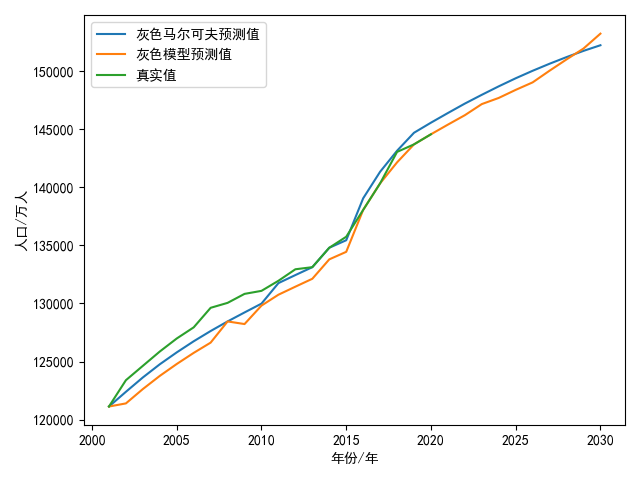
\includegraphics[width=.8\textwidth]{figures/ads.png}
			\caption{人口总数预测对比曲线图
			}\label{lcdadasdat}
		\end{figure}
	
	
	
	由图~\ref{lcdadasdat}~中的预测解曲线直观对比可知,由马尔科夫模型校正后的预测值相较于传统灰色预测值的\textbf{拟合度更高},波动性一致,且较于传统灰色模型预测值更能反应实际值的波动。两种模型预测指标如表~\ref{jjj}~所示:
	
	\begin{table}[H]
		\centering\caption{预测结果检验}\label{jjj}
		\begin{tabular}{cccc}
			\toprule[1.5pt]
			\multicolumn{1}{m{6cm}}{\centering 检验参数}
			& \multicolumn{1}{m{2cm}}{\centering RMSE}
			& \multicolumn{1}{m{2cm}}{\centering MAPE}
			& \multicolumn{1}{m{2cm}}{\centering NSE}
			\\
			\midrule[0.5pt]	
			传统灰色预测数值 &   30040.04 &  0.0213 & 0.9455\\ 
			灰色马尔科夫预测数值&  12838.64  &  0.0095  &  0.9900 \\  
			\bottomrule[1.5pt]	
		\end{tabular}
	\end{table} 
	
	从上述的预测结果可以得出:利用灰色马尔科夫模型修正后求出的人口总数的均方根误差值RMSE都小于传统灰色模型,表明\textbf{校正后结果可靠性更高}。且修正后模型MPAE值较于传统模型更接近$0$,NSE值更接近 $1$,说明改进后的灰色马尔科夫模型的\textbf{拟合程度更高},\textbf{预测效果更好},适用于人口的短期预测。
	
		
        \subsection{实验结果分析}
  
  根据灰色马尔可夫模型预估出$ 2021-2030$ 年全国人口总数如表~\ref{biaaddao1}~所示。由于符合全面二孩政策的目标人群较多,历史累积的潜在生育能量较大,政策放开后,会导致年度出生人口和妇女时期生育水平的急剧增加和波动,从而影响中国未来10年的总人口规模。由表~\ref{biaaddao1}~可知,从2016年全面放开二孩后,中国总人口迅速增加,到2020年,总人口最低估计14.558亿,最高估计14.688亿,人口均值为14.623亿;到2030年,总人口最低估计增加到15.225亿,最高估计增至15.355亿,人口均值达到15.29亿。
  
 		\begin{table}[H]
 	\setstretch{1}  %设置表的行间距
 	\centering		
 	\caption{面放开二孩后15年(2016-2030年)中国总人口预测结果}\label{biaaddao1}
 	\begin{tabular}{cccccc}
 		\toprule[2pt]
 		\multicolumn{1}{m{2cm}}{\centering 年份}
 		& \multicolumn{1}{m{2cm}}{\centering 人口}
 		&\multicolumn{1}{m{2cm}}{\centering 年份}
 		& \multicolumn{1}{m{2cm}}{\centering 人口}
 		&\multicolumn{1}{m{2cm}}{\centering 年份}
 		& \multicolumn{1}{m{2cm}}{\centering 人口}
 		\\
 		\midrule[1pt]
 		2001 & 	121121&2011 &130756&2021 &146413\\ 
 		2002	& 122389 & 2012 &131448 &2022& 147226\\
 		2003&  123626&  2013& 132129&2023& 147982\\
 		2004& 124761 & 2014 &132802 &2024&148713 \\
 		2005	&125786  & 2015 & 133450&2025& 149407\\
 		2006&126743  & 2016 &139063  &2026&150053\\
 		2007& 127627 & 2017 &141352&2027&150661\\
 		2008&128453  & 2018 & 143161&2028& 151231\\
 		2009&  129227&  2019& 144712&2029& 151768\\
 		2010 & 	129988&2020 &145581&2030& 152253\\ 
 		\bottomrule[2pt]	
 	\end{tabular}
 \end{table}
 
  从人口的增长速度来看,全面放开二孩前,2010-2015年的人口年均增长率为6.1\%,全面放开二孩后,以人口估计均值为例,2015-2020年的人口年均增长率为12.5\%,2020-2025年为5.2\%,2025-2030年为3.8\%,2015-2030年为7.2\%。可以看出,全面放开二孩后,中国总人口的增长速度呈现“快升快降”的增长规律,并且放开后的整体增长速度快于放开前的增长速度。

  
  
\begin{figure}[H]
  	\centering
  	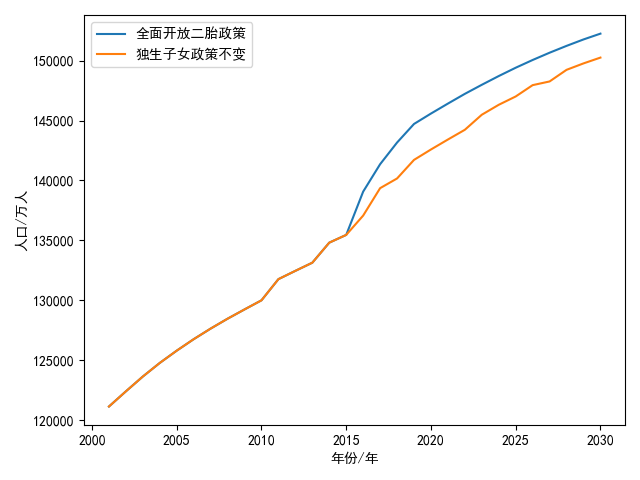
\includegraphics[width=\textwidth]{figures/da.png}
  	\caption{放开二孩政策前后(2001-2030年)中国人口总量变化趋势对比}\label{lsdasdsssct}
  \end{figure}
    
  为进一步刻画全面放开二孩对中国总人口的影响,根据2010年全国人口普查资料及历年中国统计年鉴的数据,通过队列要素法模拟了生育政策维持不变情况下的人口未来走势,并将其与全面放开二孩条件下的人口未来走势(估计均值,下同)进行对比。由图~\ref{lsdasdsssct}~可以看出,若维持独生子女生育政策不变,到2030年中国总人口仍会持续增加,但增加的速度和幅度都逐渐放缓,2020年将达到14.093亿,到2030年将达到14.523亿。全面放开二孩后,可明显地改变中国未来人口的发展轨迹,在一定时期内提升人口增加的速度和幅度。到2020年,总人口达到14.623亿,比维持政策不变多出5300万;到2030年,总人口将达到15.29亿,比维持政策不变多出7670万,差异十分明显。再从2030年以后人口的走势来看,若维持政策不变,中国将马上进入人口负增长时期,而全面放开二孩可以有效地延缓中国总人口的递减趋势。但从另一个角度来看,全面放开二孩后多出生的人口也将给中国未来的资源环境产生更大的压力,并对就业、基础设施和公共服务设施等产生更大的需求,这些都应该成为未来制定相关政策必须考虑的重要因素。
  
  
	\section{问题二模型的建立与求解}
		\subsection{问题描述与分析}
		问题二要求建立适当的人口数学模型,并利用模型对某地区或区域人口结构及变化进行预测分析。
		
		针对人口预测和人口控制问题,可以建立偏微分方程模型,并推导死亡率、生育率函数等参数方程,从而实现出生率、死亡率、老龄化指数、劳动力指数等参数的预测。此外,将偏微分方程模型视作动力模型,还可以用控制论的观点看待人口问题,将最优控制理论等方法用于人口系统。
		
		本文在分析死亡、出生、迁移三种因素的基础上推导离散形式的人口发展方程,考察不同年龄段人口变化。此外,自改革开放以来,市场经济规律作用下的迁移对人口发展方程影响越来越大,故本文建立基于动力系统城乡迁移人口流动规律的带有迁移项的$Leslie$人口发展模型,设计使用免疫差分进化算法,估计$Leslie$模型中城市化水平、人口迁移率等未知参数。
			
			
    	其思维流程图如图~\ref{lssssct}~所示:

			\begin{figure}[H]
				\centering
				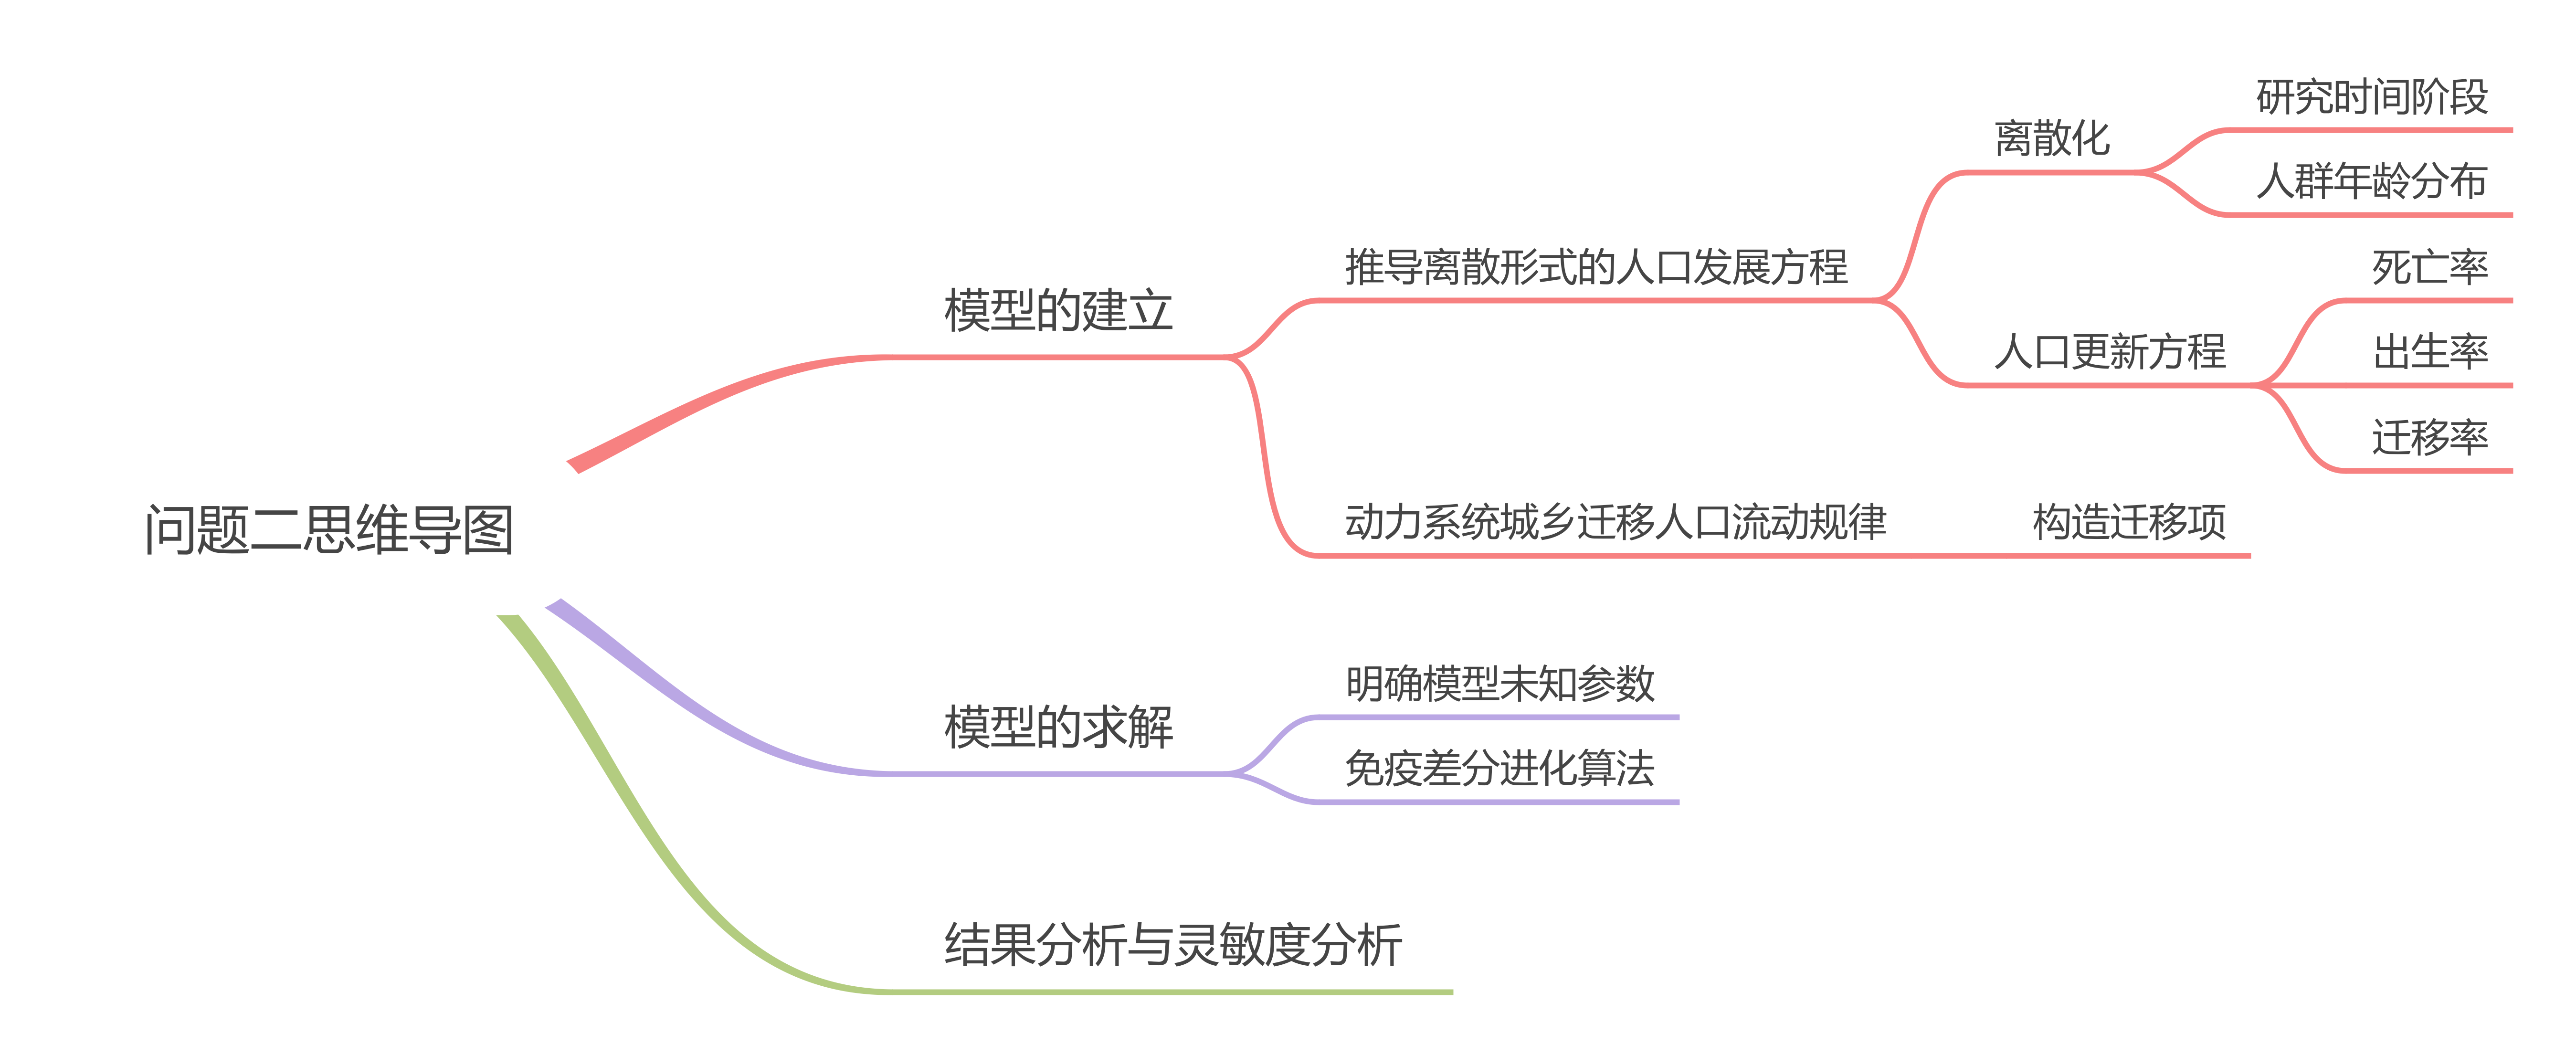
\includegraphics[width=\textwidth]{figures/kkks.png}
				\caption{问题二思维流程图}\label{lssssct}
			\end{figure}

		\subsection{Leslie人口模型建立}
		
		考虑人口的死亡、出生、迁移等因素,基于已有的$Leslie$模型,推导人口发展离散方程,建立带有迁移项的$Leslie$人口发展模型。
		
		分别以一年和一岁为步长离散化研究时间阶段和人群年龄分布。将总人口按年龄划分为$n$组,即$0$到$n-1$岁各一组,$n$岁以上人群为一组,共$n+1$组。定义$p(t)$是研究时间阶段的第$t$年满$i$周岁,但不满$i+1$周岁的人口数。记第$t$年人口分布为
		\begin{gather}
		P(t)=(p_0(t),p_1(t),...,p_{n}(t))^T.
		\end{gather}
		
		记第$t$年年龄为$i$岁的人群死亡率为$d_i(t)$。则单独考察人口发展过程中的死亡率时,第$t$年年龄为$i$岁的人群(第$i+1$组)在第$t+1$年仍然存活的人数为$(1-d_i(t))p(t)$。则仅考虑死亡率时,第$t+1$年人口在第$t$年基础上更新为
		\begin{gather}
		W(t)P(t)=(0,[1-d_0(t)]p_0(t),...,[1-d_{n-1}(t)]p_{n-1}(t)+[1-d_{n}(t)]p_{n}(t))^T,
		\end{gather}
		其中,$W(t)$是构造的使得等式成立的关系矩阵,满足
		\begin{gather}
		W(t)=\begin{pmatrix}
		0 & 0 & \cdots  & 0 & 0\\ 
		1-d_1(t) & 0 & \cdots  & 0 & 0\\ 
		0 & 1-d_1(t) & \cdots  & 0  & 0\\ 
		\vdots  & \vdots  & \ddots  & \vdots & \vdots\\ 
		0 & 0 & \cdots  & 1-d_1(t) & 1-d_1(t)
		\end{pmatrix}.
		\end{gather}
		
		当仅考虑生育率对人口发展的影响时,新增人口来源是总人口中存活的处于适育年龄的女性生育的新生儿。定义第$t$年年龄为$i$岁的人群中女性占比为$k_i(t)$,生育模式为$h_i(t)$,$\beta(t)$为女性平均生育率,记$[r_1,r_m]$是女性适育区间。则第$t+1$年出生率可以表示为
		\begin{gather}
		b_{r(i)}(t)=[1-d_{r(i)}(t)]k_{r(i)}(t)h_{r(i)}(t),
		\end{gather}
		其中,\begin{gather}
		r(i)=\left\{\begin{matrix}
		i,r_1 \leq i\leq r_m,
		\\ 
		0,otherwise.
		\end{matrix}\right.
		\end{gather}
		
		单独考虑城市化导致的人口迁入迁出,净迁徙人数可以表示为
		\begin{gather}
		v_i(t)=[r(t+1)-r(t)]\cdot \sum_{i=1}^{n}[p_i^1(t)+p_i^2(t)]f_i(t),
		\end{gather}
		其中,$r(t)$是城市人口占总人口的比例,反映城市化水平。$f_i(t)$是迁徙人口的比例。
		
		综合死亡率、出生率、迁徙率,添加迁移项的$Leslie$模型可以表示为
		\begin{gather}
		\left\{\begin{matrix} 
		P^k(t+1)=W^k(t)P^k(t)+\beta(t)B^k(t)P^k(t)+(-1)^{k+1}V(t),\\ 
		P^k(0)=(p^k_0(0),p^k_1(0),...,p^k_{n}(0))^T.
		\end{matrix}\right.
		\end{gather}
		

		\subsection{免疫差分进化算法}
		%\paragraph{初始化}
		本文设计免疫差分进化算法估计添加迁移项的$Leslie$模型中的未知参数,定义决策向量为
		\begin{gather}
		X=[x_1,x_2,x_3,x_4,x_5,x_6],
		\end{gather}
		其中$x_1$、$x_2$、$x_3$、$x_4$、$x_5$和$x_6$分别表示城市人口占总人口比率、人口迁移率、女性平均生育率、城市乡村人口死亡率、生育模式系数以及女性占。将目标函数定义为损失函数如下
		\begin{gather}
		\sum_{t=1}^{T}\sum_{i=1}^{n}(p_i(t)-\hat{p}_i(t))^2,
		\end{gather}
		其中$T$表示选取数据的终止节点,即表示选取用于估计参数的数据来自研究人口发展变化规律的第$1$天到第$T$天。损失函数$Loss$表示预测结果与实际结果间的距离,即$Loss$值越小,预测曲线就与真实曲线越接近。
		\paragraph{种群初始化}
		在解空间中随机产$p$个初始个体$
		X_i(0)=[x_1,x_2,x_3,x_4],(i=1,2,3,\cdots,p).
		$
		其中第$i$个个体的第$j$维取值方式如下
		\begin{gather*}
		x_{i,j}(0)=x_{j,min}+rand(0,1)(x_{j,max}-x_{j,min}),\\i=1,2,3,\cdots,p,j=1,2,3,4,
		\end{gather*}
		其中$p$表示种群规模,$x_{j,max}$和$x_{j,min}$分别表示决策变量$X$第$j$维的
		取值范围上界与下界。
		\paragraph{变异}
		在第$g$次迭代中,生成变异个体$H_i(g)$,从种群中随机选取三个个体$X_{p1}(g)$,$X_{p2}(g)$和$X_{p3}(g)$,且$p_1\neq p_2\neq p_3\neq i$,生成的变异向量为
		\begin{gather*}
		H_i(g)=X_{p1}(g)+F(g)*(X_{p2}(g)-X_{p3}(g)),
		\end{gather*}
		$F(g)\in (0,1)$是每一代中的放缩因子,其服从柯西分部如下
		\begin{gather*}
		F(g)=cauchyrnd(uF,0.1),
		\end{gather*}
		其中$uF$是$F$的期望值,本文取值为$uF=0.5$。
		\paragraph{交叉}
		对第$g$代种群中第$i$个体进行交叉操作,生成交叉个体$V_i(g)$,具体表达式如下:
		\begin{gather}
		v_{i,j}=\left\{\begin{matrix}h_{i,j}(g),rand(0,1)\leq cr_{i},
		\\ x_{i,j}(g),rand(0,1)>cr_{i},
		\end{matrix}\right.
		\end{gather}
		其中$cr_{i}\in[0.1,0.6]$是个体$i$的交叉概率,参数$cr_{i}$将进行自适应调整,具体表达式如下:
		\begin{gather}
		cr_{i}=\left\{\begin{matrix}cr_{l}+(cr_{u}-cr_{l})\frac{Loss_{i}-Loss_{min}}{Loss_{max}-Loss_{min}} , Loss_{i}>\overline{Loss},
		\\ cr_{l},Loss_{i}\leqslant  \overline{Loss}.
		\end{matrix}\right.
		\end{gather}
		\paragraph{免疫选择}
		混合第$g$代的交叉个体$V(g)$与原始个体$X(g)$,得到待选组$\left \{ X '(g+1)\right \}$如下
		\begin{gather*}
		X_i '(g+1)=\left\{\begin{matrix}  X_i (g),i\leqslant p,
		\\  V_{i-p} (g),i>p.
		\end{matrix}\right.
		\end{gather*}
		
		个体 $X_a '(g+1)$和$X_b '(g+1)$的亲和度$S_{a,b}$可表示为
		\begin{gather}
		S_{a,b}=\sqrt{\sum _{i=1}^6( \frac{x_{i,a}-x_{i,b}}{x_{i,max}-x_{i,min}})^2},
		\end{gather}
		$S_{a,b}$为$X_a '(g+1)$和$X_b '(g+1)$的归一化距离,表示个体$X_a '(g+1)$和$X_b '(g+1)$的相似性。定义个体$X_i '(g+1)$的抗体浓度为$C_{i}$,即
		\begin{gather*}
		C_{i}=\frac{1}{2p}\sum _{j=1}^{2p} N_{i,j},\\
		N_{i,j}=\left\{\begin{matrix}1,S_{i,j}\geqslant \mu ,
		\\ 0,S_{i,j}< \mu ,
		\end{matrix}\right.
		\end{gather*}
		$\mu(\mu\in[0,1])$为相似度阈值,即当个体$i$和$j$的亲和度$S_{i,j}\geqslant \mu$时认为个体$i$和$j$为相似个体。$C_{i}$即为$\left \{ X '(g+1)\right \}$中$X_i '(g+1)$的相似个体所占比例,$C_{i}$越大即表示$X_i '(g+1)$所在区域的个体密度越大。我们优先将损失函数$Loss$值最优的前$\sigma$个解放入下一代个体$\left \{ X(g+1)\right \}$中以防止最优解丢失。再计算剩余个体的复合适应度函数,即个体$i$的复合适应度函数可表示为
		\begin{gather}
		min F(X_i '(g+1))=\frac{Loss(X_i '(g+1))-Loss_{min}}{Loss_{max}-loss_{min}}+C_{i},
		\end{gather}
		即选取复合适应度函数$F$较优的剩余$p-\sigma$个个体放入下一代个体$\left \{ X(g+1)\right \}$中。重复迭代上述算法$G$次后终止算法并输出最优参数集$X_{best}$。
        \subsection{实验结果及分析}
        实验选取厦门人口数目,使用免疫差分进化算法可求得厦门的未统计参数如表~\ref{sda}~所示 
		 		\begin{table}[H]
			\setstretch{1}  %设置表的行间距
			\centering		
			\caption{免疫差分进化算法求得的未统计参数
			}\label{sda}
			\begin{tabular}{ccc}
				\toprule[2pt]
				\multicolumn{1}{m{4cm}}{\centering 参数名称}
				& \multicolumn{1}{m{3cm}}{\centering 符号}
			& \multicolumn{1}{m{3cm}}{\centering 值}
				\\
				\midrule[1pt]
				出生率 & 	$\lambda_1$, $\lambda_2$&0.0326, 0.0435\\ 
				男性出生比率 &$\aleph_1$, $\aleph_2$&0.535, 0.547\\ 
				转化率 &$x_1$, $x_2$&0.009, 0.011\\
				城镇女性死亡率 &$\delta_1$, $\delta_2$&0.00073, 0.00068\\  
				城镇男性死亡率 &$\delta_3$, $\delta_4$&0.00068, 0.00057\\  
				农村女性死亡率 &$\delta_5$, $\delta_6$&0.00113, 0.00097\\  
				农村男性死亡率 &$\delta_7$, $\delta_8$&0.00104, 0.00089\\  
				\bottomrule[2pt]	
			\end{tabular}
		\end{table}

现阶段我国生育水平的不稳定性,根据建立的Leslie模型,运用MATLAB软件计算出2000年到2050年我国育龄妇女(15-49岁)人口,并做出的散点图如下:
			\begin{figure}[H]	
	\centering
	\subfigure{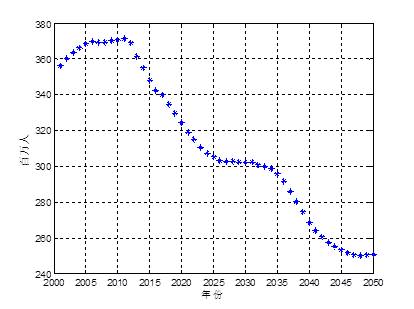
\includegraphics[height=6cm,width=7.5cm]{figures/adasd.png}}
	\subfigure{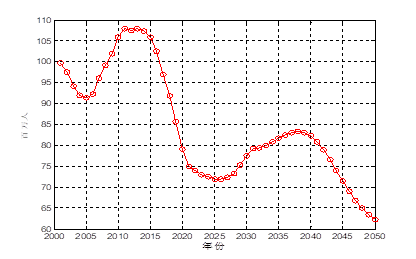
\includegraphics[height=6cm,width=7.5cm]{figures/qefeqf.png}}
	\caption{未来我国育龄妇女(15-49岁)人口预测 }\label{lssdaddaassct}
	\label{fisg}
\end{figure}


从图~\ref{lssdaddaassct}~中可以看出我国育龄妇女(15-49岁)人口在2010年左右到达到高峰,从图~\ref{lssdaddaassct}~我们发现,我国生育旺盛期育龄妇女(20-29)人数在2012年将达到高峰,到2025年左右有进入一个小低谷,然后再2037年左右有达到一个小高峰。第二个我国生育旺盛期育龄妇女(20-29)人数小高峰的原因在于在2012年人口出生高峰期的女婴到2037年时达到生育旺盛期,因此,在2025年生育旺盛期育龄妇女(20-29)人数达到低谷时有回升的形势。


\section{灵敏度分析}

在不同的总合生育率 下按照前面的方法分别计算从2001年到2050年全国人口总数的预测值,并画出图形如图~\ref{lssdassct}~所示


\begin{figure}[H]
	\centering
	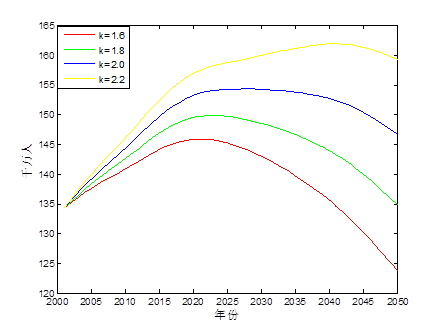
\includegraphics[width=\textwidth]{figures/das.png}
	\caption{在不同的k值下对各年份全国总人口数的预测 }\label{lssdassct}
\end{figure}

由图~\ref{lssdassct}~可以看出当 值很小时人口增长比较缓慢,达到峰值后人口数量很快下降出现严重负增长;当 值很大时人口增长速度很快,达到峰值后下降的速度缓慢,在此情况下人口数量急剧膨胀。只有当 值适中时,总人口增长才比较稳定。


在不同的总和生育率 下按照前面的方法分别计算从2001年到2050年全国老龄化变化趋势,并画出图形如图~\ref{lsssdsasct}~所示

\begin{figure}[H]
	\centering
	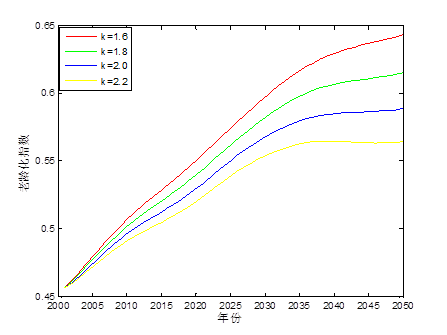
\includegraphics[width=\textwidth]{figures/ad.png}
	\caption{在不同的k值下对各年份老龄化变化趋势}\label{lsssdsasct}
\end{figure}

由图~\ref{lsssdsasct}~可以看出 值越小,老龄化增大的速度越快; 值越大老龄化指数增长平缓年龄结构稳定,有利于社会发展。
由以上分析可知国家在制定人口政策时要多方面考虑,如果只看重对人口总数的控制可能导致社会老龄化严重、劳动力不足这显然是不利于社会经济发展的;相反如果为了防止社会老龄化加快而放任人口的增长,也会导致社会人口过多对资源和环境带来巨大压力。因此只有掌握好一个“平衡点”正确制定政策才能使国民经济持续增长,人民生活水平不断提高。


    \section{结论与政策建议}
\textbf{    致卫生健康委员会相关部门的一封信:}
    
    
        在经历了迅速从高生育率到低生育率的转变之后,我国人口的主要矛盾已经不再是增长过快,而是人口红利消失、临近超低生育率水平、人口老龄化、出生性别比失调等问题。
        第一,我国人口仍然是持续的低速增长,但二
        孩政策能使得出生人口增加,延缓人口金字塔的
        收缩型发展趋势。在全面二孩政策实施后,不同生
        育率(生育意愿)假设下的悲观情形、折衷情形、乐
        观情形的人口峰值到来时间点和峰值有所不同。
        生育意愿越强,峰值越高,峰值来的时间越晚,即
        放开二孩、刺激生育的政策是能够刺激我国的人
        口增长的,并能通过刺激新生儿的增长,在一定程
        度上改善我国的人口结构。但是,无论何种情形,
        对人口发展的长期趋势是不可扭转的,在达到峰
        值后,人口规模下降。
        
        第二,生育政策的改变在短期内对劳动人口
        不产生影响,但在长期具有一定的影响。这是因为
        这一政策具有时滞性:“二孩”从婴儿成长为适龄
        劳动力并成功就业的这一过程是漫长的,毛春梅
        (2016)认为这需要 15 到 20 年,故在 2030 年前,
        无论是何种情形的二孩政策均对原有生育模式下
        的劳动人口数不产生影响。人口规模在长期是下
        降趋势,劳动人口数量也呈下降趋势,但不同情形
        下的劳动人口数量还是存在差别。
        
        第三,根据抚养比分析,全面二孩政策对降低
        抚养比,带来新一轮的人口红利的作用极其微小,
        人口福利或将在 2028 年消失,为此,我们应积极
        应对,寻找其他的解决方法。但是,基于家庭层面分
        析,全面二孩政策可以彻底终止“421”家庭结构,而
        二孩的本身也是一种变相的养老,故它也可以获得
        更多的家庭养老支持,彻底避免“失独”风险,从而
        维持并增强家庭幸福感,实现社会稳定发展。
        
        从整体上说,无论人们的生育意愿或高或低,
        实施二孩政策是符合经济发展和社会和谐的,是
        利大于弊的。虽短期内(2035 年前)效果不明显,但
        长期而言,是可以增加劳动人口、改善家庭结构和
        人口结构、缓和我国当前“未富先老”的悲剧、延缓
        我国老龄化进程。
        
        但是,全面二孩政策的实施效果受到众多因
        素的影响,根据预测结果来看,不同的生育意愿情
        形在长期内对整个政策的效果产生较大的影响,
        为保证政策实施效果,本文建议,在政策的后续实
        施中,通过补贴、税收等手段刺激人们的生育意
        愿,同时强化教育改革,强调驾驭的普惠性,让教育
        普民惠民,让每一个家庭都能负担其教育,每一个
        孩子都能通过教育成才,更好地参与劳动力竞争。

  以上建议仅供参考,不足之处请予以批评指正。
%  	\section{灵敏度分析}
 
  	\section{模型的评价}
		\subsection{模型的优点}
			\begin{itemize}                                             
			\item [(1)]利用马尔可夫模型改进后的灰度预测值与实际值拟合度更高,波动性保持一致,预 测的效果更好。 
			\item [(2)] 结合了人口迁移的实际特点改进了 Leslie人口模型,且使用免疫差分进化算法估计参数, 使得预测模型更贴近于我国的实际情况。
			\end{itemize}
		\subsection{模型的缺点}
问题一中的灰色预测模型只能做短期预测,并不适用于长期预测。

 
	\newpage	%换页符
	%%参考文献
	%\begin{thebibliography}{9}%宽度9
	% \setlength{\itemsep}{-2mm}
		\addcontentsline{toc}{section}{参考文献}
	\nocite{*}		%排版未引用的参考文献
	\begin{thebibliography}{9}%宽度9
		\bibitem{1}Liu M. Dynamics of a stochastic regime-switching predator–prey model with modified Leslie–Gower Holling-type II schemes and prey harvesting[J]. Nonlinear Dynamics, 2019, 96(1): 417-442.
		\bibitem{2}严政人, 魏玉蕊, 陈庆炜. 基于 Leslie 模型分析 “全面二孩” 政策对人口数量影响[J]. 现代信息科技, 2016, 36(7): 44-47.
		\bibitem{3}吴逸飞, 许亦楷, 李卓明. 基于误差修正模型和 Leslie 模型的 “全面二胎” 政策影响研究[J]. 人力资源管理 (汉), 2017 (6): 304-307.
		\bibitem{4}张和平, 陈齐海. 基于灰色马尔可夫模型的网络舆情预测研究[J]. 情报科学, 2018, 36(1): 75-79.
		\bibitem{5}汤银英, 李龙, 秦阳. 基于改进型灰色马尔可夫模型的公路货运价格预测[J]. 交通运输工程与信息学报, 2018, 16(1): 38-43.
	\end{thebibliography}

	\newpage
	%附录
	\appendix %%附录
	\section{代码}
		\subsection*{灰色马尔可夫模型--matlab源代码}
		\begin{lstlisting}[language=matlab]
		x = [970279 1259308 1127571 1163959 1169540 1076938 991350 953275 951508 904434 889381 864015 836236];
		
		%二次拟合预测GM(1,1)模型
		sizexd2 = size(x,2);
		%求数组长度
		
		k=0;
		for y1=x
		k=k+1;
		if k>1
		x1(k)=x1(k-1)+x(k);
		%累加生成
		z1(k-1)=-0.5*(x1(k)+x1(k-1));   
		%z1维数减1,用于计算B
		yn1(k-1)=x(k);
		else
		x1(k)=x(k);
		end
		end
		%x1,z1,k,yn1
		
		sizez1=size(z1,2);
		%size(yn1);
		z2 = z1';
		z3 = ones(1,sizez1)';
		
		YN = yn1';   %转置
		%YN
		
		B=[z2 z3];
		au0=inv(B'*B)*B'*YN;
		au = au0';
		%B,au0,au
		
		afor = au(1);
		ufor = au(2);
		ua = au(2)./au(1);
		%afor,ufor,ua 
		%输出预测的  a u 和 u/a的值
		
		constant1 = x(1)-ua;
		afor1 = -afor;
		x1t1 = 'x1(t+1)';
		estr = 'exp';
		tstr = 't';
		leftbra = '(';
		rightbra = ')';
		%constant1,afor1,x1t1,estr,tstr,leftbra,rightbra
		
		strcat(x1t1,'=',num2str(constant1),estr,leftbra,num2str(afor1),tstr,rightbra,'+',leftbra,num2str(ua),rightbra)
		%输出时间响应方程
		
		%******************************************************
		%二次拟合
		
		k2 = 0;
		for y2 = x1
		k2 = k2 + 1;
		if k2 > k  
		else
		ze1(k2) = exp(-(k2-1)*afor);  
		end
		end
		%ze1
		
		sizeze1 = size(ze1,2);
		z4 = ones(1,sizeze1)';
		G=[ze1' z4];
		X1 = x1';
		au20=inv(G'*G)*G'*X1;
		au2 = au20';
		%z4,X1,G,au20
		
		Aval = au2(1);
		Bval = au2(2);
		%Aval,Bval
		%输出预测的  A,B的值
		
		strcat(x1t1,'=',num2str(Aval),estr,leftbra,num2str(afor1),tstr,rightbra,'+',leftbra,num2str(Bval),rightbra)
		%输出时间响应方程
		
		nfinal = sizexd2-1 + 3;
		%决定预测的步骤数5  这个步骤可以通过函数传入
		
		%nfinal = sizexd2 - 1 + 1;
		%预测的步骤数 1
		
		for  k3=1:nfinal
		x3fcast(k3) = constant1*exp(afor1*k3)+ua;
		end
		%x3fcast
		%一次拟合累加值
		
		for  k31=nfinal:-1:0
		if k31>1
		x31fcast(k31+1) = x3fcast(k31)-x3fcast(k31-1);
		else
		if k31>0
		x31fcast(k31+1) = x3fcast(k31)-x(1);
		else
		x31fcast(k31+1) = x(1);
		end
		end
		
		end
		x31fcast
		%一次拟合预测值
		
		
		for  k4=1:nfinal
		x4fcast(k4) = Aval*exp(afor1*k4)+Bval;
		end
		%x4fcast
		
		for  k41=nfinal:-1:0
		if k41>1
		x41fcast(k41+1) = x4fcast(k41)-x4fcast(k41-1);
		else
		if k41>0
		x41fcast(k41+1) = x4fcast(k41)-x(1);
		else
		x41fcast(k41+1) = x(1);
		end
		end
		
		end
		x41fcast,x
		%二次拟合预测值
		
		%***精度检验p C************//////////////////////////////////
		k5 = 0;
		for y5 = x
		k5 = k5 + 1;
		if k5 > sizexd2  
		else
		err1(k5) = x(k5) - x41fcast(k5);  
		end
		end
		%err1
		%绝对误差
		
		
		xavg = mean(x);
		%xavg
		%x平均值
		
		err1avg = mean(err1);
		%err1avg
		%err1平均值
		
		k5 = 0;
		s1total = 0 ;
		for y5 = x
		k5 = k5 + 1;
		if k5 > sizexd2  
		else
		s1total = s1total + (x(k5) - xavg)^2;  
		end
		end
		s1suqare = s1total ./ sizexd2;
		s1sqrt = sqrt(s1suqare);
		%s1suqare,s1sqrt
		%s1suqare  残差数列x的方差  s1sqrt 为x方差的平方根S1
		
		k5 = 0;
		s2total = 0 ;
		for y5 = x
		k5 = k5 + 1;
		if k5 > sizexd2  
		else
		s2total = s2total + (err1(k5) - err1avg)^2;  
		end
		end
		s2suqare = s2total ./ sizexd2;
		%s2suqare   残差数列err1的方差S2
		
		Cval = sqrt(s2suqare ./ s1suqare);
		%nnn = 0.6745 * s1sqrt
		%Cval  C检验值
		
		k5 = 0;
		pnum = 0 ;
		for y5 = x
		k5 = k5 + 1;
		if abs( err1(k5) - err1avg ) < 0.6745 * s1sqrt
		pnum = pnum + 1;
		%ppp = abs( err1(k5) - err1avg )     
		else
		end
		end
		pval = pnum ./ sizexd2;
		
		%p检验值
		
		%arr1 = x41fcast(1:6)
		\end{lstlisting}
		
			
		\subsection*{Leslie人口模型--matlab源代码}

\begin{lstlisting}[language=matlab]
function W=compare(x)
p=0.464429182;      %女性占总人口的比例
N=[0.680891272  0.58459172  0.584558207 0.692220217 0.72411021  0.775536041 0.847368918 0.834418703 0.917922042 0.951466819 1.070015717 1.249256063 1.199263988 1.202198525 1.274218917 1.111050839 0.992314425 0.893797544 0.874657347 0.984356877 0.859576778 0.85215346  0.90864418  0.897944807 0.880539323 1.019086724 1.04218667  1.114823731 1.192867199 1.203566572 1.272973995 1.328513576 1.254992403 1.333819445 1.103186123 1.22470307  1.220643442 1.236736319 1.390726415 0.980765111 0.646684069 0.785660623 0.701627592 0.910420112 0.960157646 0.914258713 0.953980568 0.927429956 0.851007759 0.825482359 0.807942823 0.736552002 0.69043204  0.60580295  0.615510624 0.554785663 0.50370135  0.480051762 0.468722817 0.455364059 0.484386541 0.447344681 0.420164498 0.44238033  0.426529091 0.428183875 0.39132953  0.380409129 0.385339967 0.327924574 0.334697711 0.307330012 0.262864834 0.270663183 0.235872165 0.208725495 0.212001549 0.178456772 0.164260316 0.149842833 0.138734916 0.109899949 0.097358277 0.0765762   0.0638135   0.055794123 0.049396016 0.0382881   0.033544777 0.023870616 0.070211606];
N0=N';
A=eye(90);
b=[0.974906966  0.999321231 0.99772433  0.999247616 0.999567418 0.999180663 0.999887948 0.999387596 0.999618586 0.999985672 0.999389434 0.999724354 0.999801796 0.999627626 0.999704795 0.999639686 0.999728462 0.999974533 0.999173327 0.998954118 0.999441067 0.999357392 0.999290675 0.998999176 0.999881604 0.998896347 0.998355939 0.999135339 0.999074527 0.998872652 0.999180794 0.998918159 0.999046112 0.999042354 0.999396027 0.998624972 0.998252716 0.999597855 0.998710945 0.999003274 0.999443444 0.999141415 0.998772101 0.998940505 0.997905005 0.998374562 0.997783774 0.997596666 0.997344906 0.996954499 0.996669784 0.996030759 0.995006639 0.996157488 0.994647744 0.995779435 0.995652313 0.99577713  0.992477806 0.994969564 0.988130537 0.989284868 0.988703961 0.988302563 0.98420824  0.984495416 0.985298735 0.980062089 0.978928307 0.977358446 0.971126989 0.969303899 0.969979818 0.96405059  0.961740312 0.96729706  0.948302346 0.946571559 0.949641387 0.935949391 0.912489482 0.9261805   0.923757863 0.928757906 0.918230333 0.887761389 0.885306858 0.875178086 0.882495752 0.824428701];
b1=[0.974906966 0.999321231 0.99772433  0.999247616 0.999567418 0.999180663 0.999887948 0.999387596 0.999618586 0.999985672 0.999389434 0.999724354 0.999801796 0.999627626 0.999704795 0.999639686 0.999728462 0.999974533 0.999173327 0.998954118 0.999441067 0.999357392 0.999290675 0.998999176 0.999881604 0.998896347 0.998355939 0.999135339 0.999074527 0.998872652 0.999180794 0.998918159 0.999046112 0.999042354 0.999396027 0.998624972 0.998252716 0.999597855 0.998710945 0.999003274 0.999443444 0.999141415 0.998772101 0.998940505 0.997905005 0.998374562 0.997783774 0.997596666 0.997344906 0.996954499 0.996669784 0.996030759 0.995006639 0.996157488 0.994647744 0.995779435 0.995652313 0.99577713  0.992477806 0.994969564 0.988130537 0.989284868 0.988703961 0.988302563 0.98420824  0.984495416 0.985298735 0.980062089 0.978928307 0.977358446 0.971126989 0.969303899 0.969979818 0.96405059  0.961740312 0.96729706  0.948302346 0.946571559 0.949641387 0.935949391 0.912489482 0.9261805   0.923757863 0.928757906 0.918230333 0.887761389 0.885306858 0.875178086 0.882495752 0.824428701 0.7717624];
for i=1:90
A(i,:)=A(i,:)*b(1,i);
end
A;         
c1=[0   0   0   0   0   0   0   0   0   0   0   0   0   0   0   4.478E-05   0.000322169 0.000358246 0.001004604 0.004683367 0.011011165 0.033616492 0.057875394 0.074871727 0.069182006 0.076039141 0.06724895  0.052429406 0.043732464 0.034350502 0.024632733 0.023252532 0.018343847 0.014701275 0.011039961 0.007117557 0.005094843 0.00359291  0.002514858 0.002484781 0.001764709 0.001471644 0.000676953 0.000265476 0.000401474 0.000408779 0.000110447 0.000192401 0.000389421 0.000224069 0   0   0   0   0   0   0   0   0   0   0   0   0   0   0   0   0   0   0   0   0   0   0   0   0   0   0   0   0   0   0   0   0   0   0   0   0   0   0   0];        %由2001年原始数据得到的生育率
t=sum(c1);
c=((x*p-t)/t+1)*c1                                %修正后的生育率
M=sum(c');                                        %总合生育率
d=zeros(91,1);
B=[c;A];
L=[B,d];                                          %构造的lestie矩阵
[V,d]=eig(L);                                     %求特征根与特征向量
p=d(42,42);                                       %特征根
Q=-V(:,42);                                       %对应的正特征向量
for i=0:49
D=L^i*N0;                                     %第i年女性人口分布
E(i+1,1)=sum(D)/p                             %第i年总人口(2001为第0年)
for j=0:90                                    %大于90岁的按90岁算
F(j+1,1)=j*D(j+1,1)/p;
T(j+1,1)=exp(-b1(1,j+1));                 
end
Y(i+1)=sum(F)/E(i+1,1);                       %平均年龄
end
Y                                                 %输出01-50年平均年龄矩阵
T=0;
s=0;
for i=0:90                                      %大于90岁的按90岁算

T=T+exp(b1(1,j+1)-1);                        %求平均寿命,不随年份而变化
end
T
W=Y/T;                                           %社会老龄化指数
x=2001:2050;
W1=compare(1.6);
W2=compare(1.8);
W3=compare(2.0);
W4=compare(2.2);
plot(x,W1,'-r')
hold on
plot(x,W2,'-G')
plot(x,W3,'-B')
plot(x,W4,'-Y')

\end{lstlisting}


\end{document}